%%=============================================================================
%% Proof of concept
%%=============================================================================
\chapter{Proof of concept}
\label{ch:proof-of-concept}

\section{Doelstelling van de PoC}

%Wat wil je bewijzen of aantonen met deze PoC?
%TODO taalcorrectie laten uitvoeren
De hoofddoelstelling van deze PoC is om na te gaan op welke manier een LLM ondersteuning kan bieden binnen een IT-supportsysteem. Er werden verschillende mogelijkheden onderzocht, maar RAG leek na analyse de meest geschikte benadering. 

%Welke hypothese test je eigenlijk?

\section{Architectuur en Ontwerp}

%Welke algemene structuur heeft je PoC?

\subsubsection{architectuur}

Deze structuur bestaat uit een graaf die is opgebouwd uit verschillende knooppunten (nodes). De graaf stelt het LLM bovendien in staat om zelfstandig te bepalen welke keuzes gemaakt moeten worden tijdens het verwerken van een vraag.

De standaard RAG architectuur gaat een query gaan embedden en haalt vervolgens de meest relevante documenten op uit de vectordatabase, zonder verdere reflectie over de nood van het ophalen van de documenten en de werkelijke relevantie van deze documenten. Hoewel dit op het eerste gezicht een efficiënte aanpak lijkt, betekent het ook dat het systeem bij elke willekeurige gebruikersvraag opnieuw de vectordatabase bevraagt, zelfs wanneer dat niet noodzakelijk is.

Om dit te vermijden, werd gebruikgemaakt van een graafstructuur die de LLM de mogelijkheid geeft om zelf te beoordelen wanneer het relevant is om deocumenten op te halen. Daarnaast wordt de LLM ook verantwoordlijk geacht om te oordelen over de opgehaalde documenten. De volledige flow van het proces kan worden bekeken in figuur~\ref{fig:flowchart}

De PoC werd uitgewerkt met behulp van Ollama, een tool waarmee open modellen lokaal kunnen worden gedraaid. Tijdens overleg met de betrokken partijen werd geen voorkeur uitgesproken voor specifieke LLM-modellen, enkel het gebruik van DeepSeek werd afgeraden.

\begin{figure}[H]
    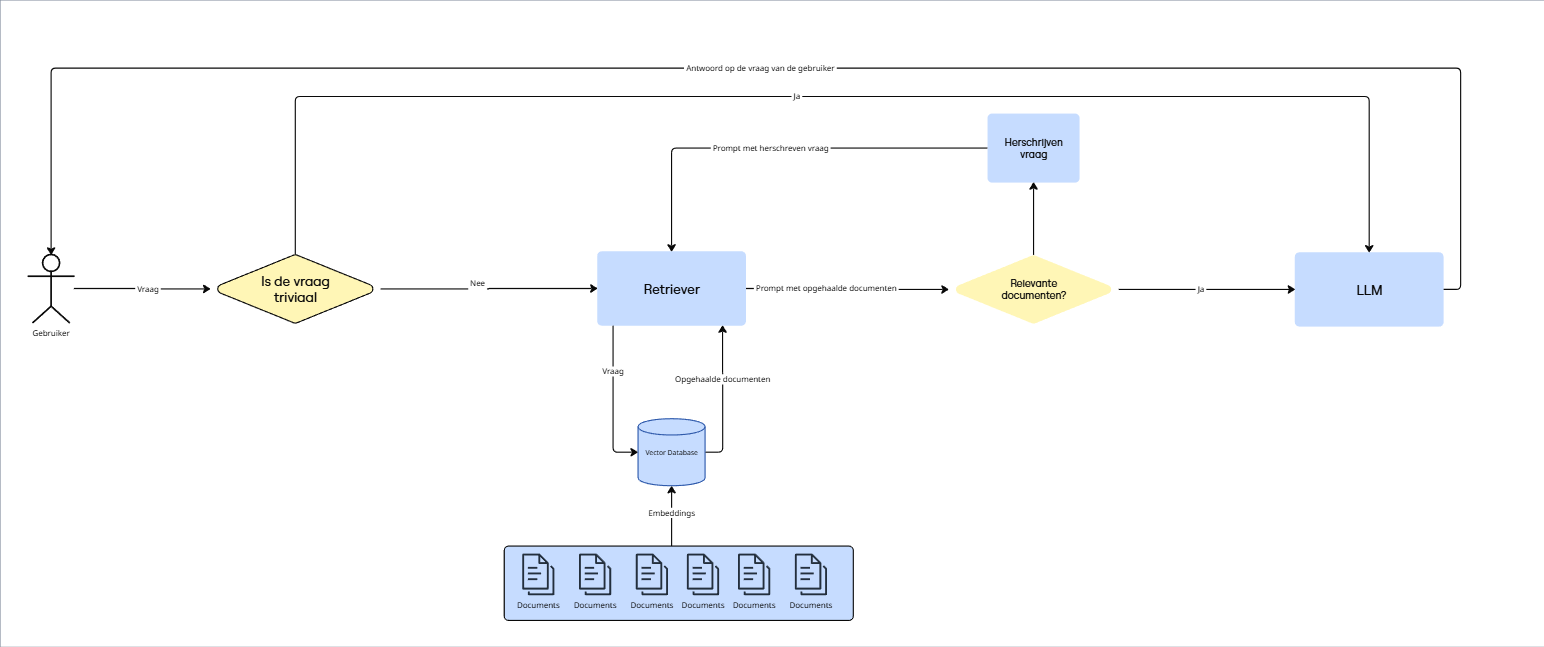
\includegraphics[width=1\textwidth]{flowchart.png}
    \caption{Visualisatie van de workflow}
    \label{fig:flowchart}
\end{figure}

%Welke tools, frameworks, programmeertalen gebruik je?

Hieronder een overzicht van de verschillende frameworks, tools en programmeertalen die werden gebruikt om deze PoC op te stellen.

Frameworks:
\begin{itemize}
    \item Langchain
    \item Langgraph
    \item Streamlit
    \item Ragaas testframework
\end{itemize}

Tools:
\begin{itemize}
    \item ChromaDB
    \item Ollama
\end{itemize}

Programeertalen:
\begin{itemize}
    \item Python
\end{itemize}

%Schema’s (bv. systeemdiagram, flowchart) zijn hier heel sterk.

\section{Implementatie}

%Hoe heb je de POC concreet opgebouwd?

De PoC werd opgebouwd volgens de klassieke RAG-implementatie. In de eerste fase werden de originele documenten opgesplitst in kleinere tekstsegmenten en vervolgens omgezet naar embeddings via een vooraf getraind embedding model. Voor deze PoC werd hiervoor gebruikgemaakt van het \textit{mxbai-embed-large model}. Van de beschikbare embedding modellen binnen Ollama biedt dit model de hoogste semantische nauwkeurigheid.

De gegenereerde embeddings worden vervolgens opgeslagen in een vectorstore. Hiervoor werd gekozen voor ChromaDB, een performante oplossing. Alternatieven zoals Faiss zijn zeker ook mogelijk.

Elke chunk heeft een grootte van 1250 karakters, met een overlap van 250 karakters tussen opeenvolgende chunks. Na het testen van verschillende chunk groottes bleek dit de kleinst mogelijke waarde te zijn waarbij nog voldoende relevante informatie kon worden opgehaald.

Deze initiële set-up maakt het mogelijk om relevante documenten snel op te halen op basis van semantische gelijkenis met de vraag van de gebruiker. Met andere woorden: dit vormt een kerncomponent van de RAG-oplossing.

%Belangrijke keuzes tijdens het bouwen (waarom bv. technologie X en niet Y?).

Belangrijkste keuzes zijn de initiële keuze voor RAG tegenover andere mogelijkheden. Eens deze keuze werd gemaakt waren verschillende mogelijkheden inzake frameworks om dit te bereiken. In deze POC werd gekozen om gebruik te maken van LangGraph. Dit is een framework waarmee zogenaamde agents kunnen worden gemaakt aan de hand van grafen. Dit is anders dan bijvoorbeeld LangChain waar je een ketting kan maken met verschillende stappen.

%Belangrijke componenten of modules kort toelichten.

\begin{lstlisting}[basicstyle=\small, frame=single, breaklines=true, postbreak=\mbox{\textcolor{red}{$\hookrightarrow$}\space}, escapeinside ={\%,}, escapechar={!}, numbers=left, language=Python, caption=Graph build]
    workflow = StateGraph(MessagesState)
    
    # Define the nodes we will cycle between
    workflow.add_node("generate_query_or_respond", generate_query_or_respond)
    workflow.add_node("tools", ToolNode([myminfin_retriever_tool]))
    workflow.add_node(rewrite_question)
    workflow.add_node(generate_answer_with_evaluation)
    
    workflow.add_edge(START, "generate_query_or_respond")
    
    # Decide whether to retrieve
    workflow.add_conditional_edges(
    "generate_query_or_respond",
    # Assess LLM decision (call `retriever_tool` tool or respond to the user)
    tools_condition
    )
    
    # Edges taken after the `action` node is called.
    workflow.add_conditional_edges(
    "tools",
    # Assess agent decision
    grade_documents_with_evaluation,
    {
        "generate_answer_with_evaluation": "generate_answer_with_evaluation",
        "rewrite_question": "rewrite_question"
    }
    )
    workflow.add_edge("generate_answer_with_evaluation", END)
    workflow.add_edge("rewrite_question", "generate_query_or_respond")
    
    # Compile
    graph = workflow.compile()
\end{lstlisting}

De volledige workflow werd gemodelleerd als een LangGraph-graaf. Deze structuur is weergegeven in figuur~\ref{fig:langgraph}.

\begin{figure}[H]
    \centering
    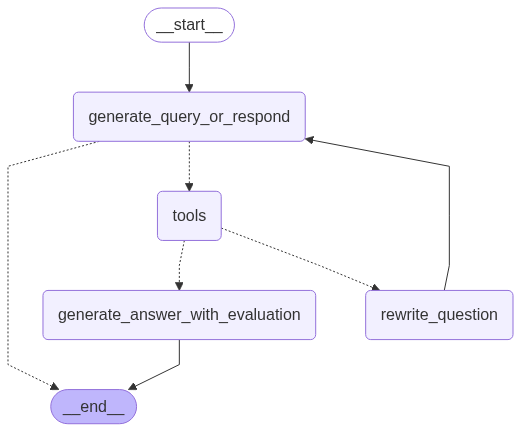
\includegraphics[width=0.8\textwidth]{langgraph_workflow.png}
    \caption{Visualisatie van de LangGraph workflow}
    \label{fig:langgraph}
\end{figure}




\section{Problemen en Oplossingen}

%Waar liep je tegenaan tijdens de implementatie?

Het kiezen van de beste technologie en wat de voor-en nadelen zijn van de verschillende zaken. Gelet op het feit dat deze frameworks vrij nieuw zijn was het moeilijk om na te gaan wat de beste te kiezen framework was om een RAG toepassing te maken

De documenten gaan parsen naar embeddings was ook een moeilijke zaak. PDF gaven niet altijd het gewenste resultaat net zoals de word documenten.
De problemen stelde zich hoofdzakelijk bij documenten die ongestructureerde elementen bevatte. Bijvoorbeeld wanneer documenten tabellen hadden werd het snel duidelijk dat de geparsde elementen van het document niet dezelfde structuur meer hadden. Een goede parsing is echter wel essentieel om een goed werkende RAG te hebben. Als de document delen geen goede structuur bevatten en vervolgens als embedding in de vector database terecht is het ook diezelfde structuur die zal worden gebruikt om toe te voegen aan de context van een LLM. Dit zorgt voor problemen bij het genereren van een antwoord, om dit op te lossen werden de eerst de documenten omgezet in eerste fase omgezet naar docx bestanden. Gelet op het feit dat ook dit niet het gewenste resultaat had werd gekozen om de bestanden om te zetten naar markdown. Dit had als voordeel dat tijdens de parsing de structuur van de documenten behouden bleef wat resulteert in een betere structuur van de relevante chunks die werden opgehaald voor het antwoorden van de LLM.

\begin{figure}[H]
    \centering
    \begin{subfigure}{0.3\textwidth}
        \centering
        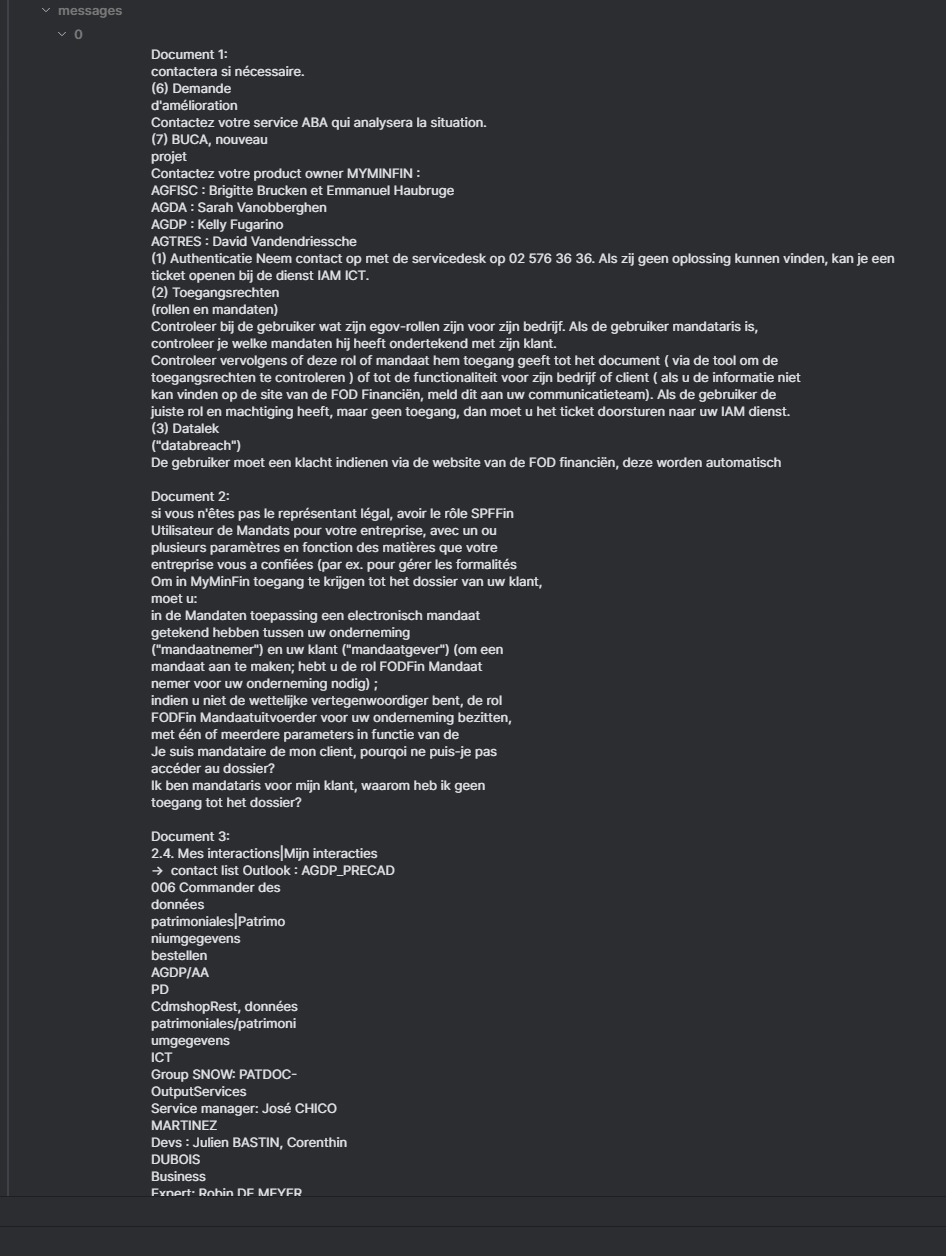
\includegraphics[width=\linewidth]{chunks_pdf.png}
        \caption{Chunks in PDF}
        \label{fig:chunks_pdf}
    \end{subfigure}
    \hfill
    \begin{subfigure}{0.3\textwidth}
        \centering
        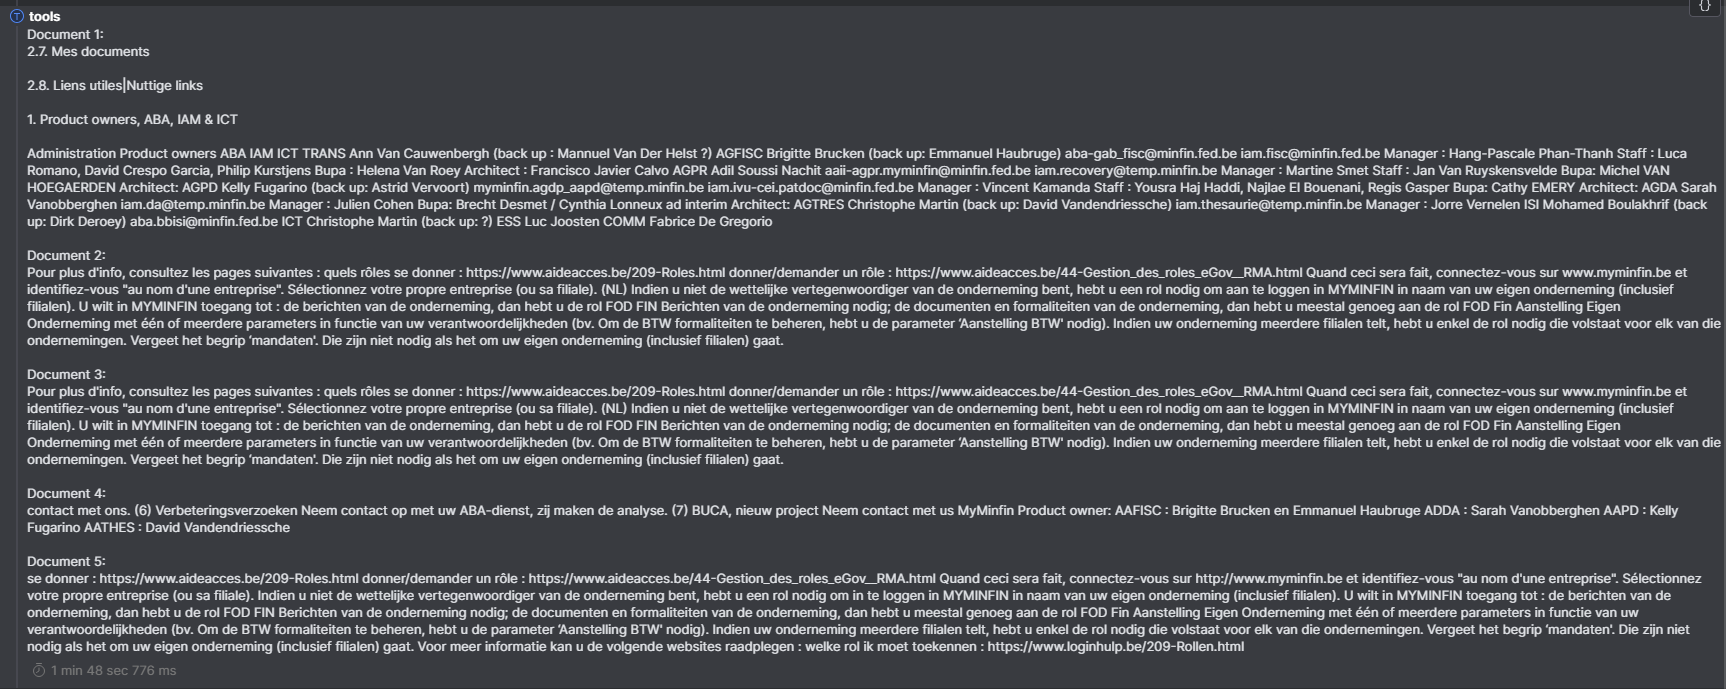
\includegraphics[width=\linewidth]{chunks_docx.png}
        \caption{Chunks in DOCX}
        \label{fig:chunks_doc}
    \end{subfigure}
     \hfill
    \begin{subfigure}{0.3\textwidth}
        \centering
        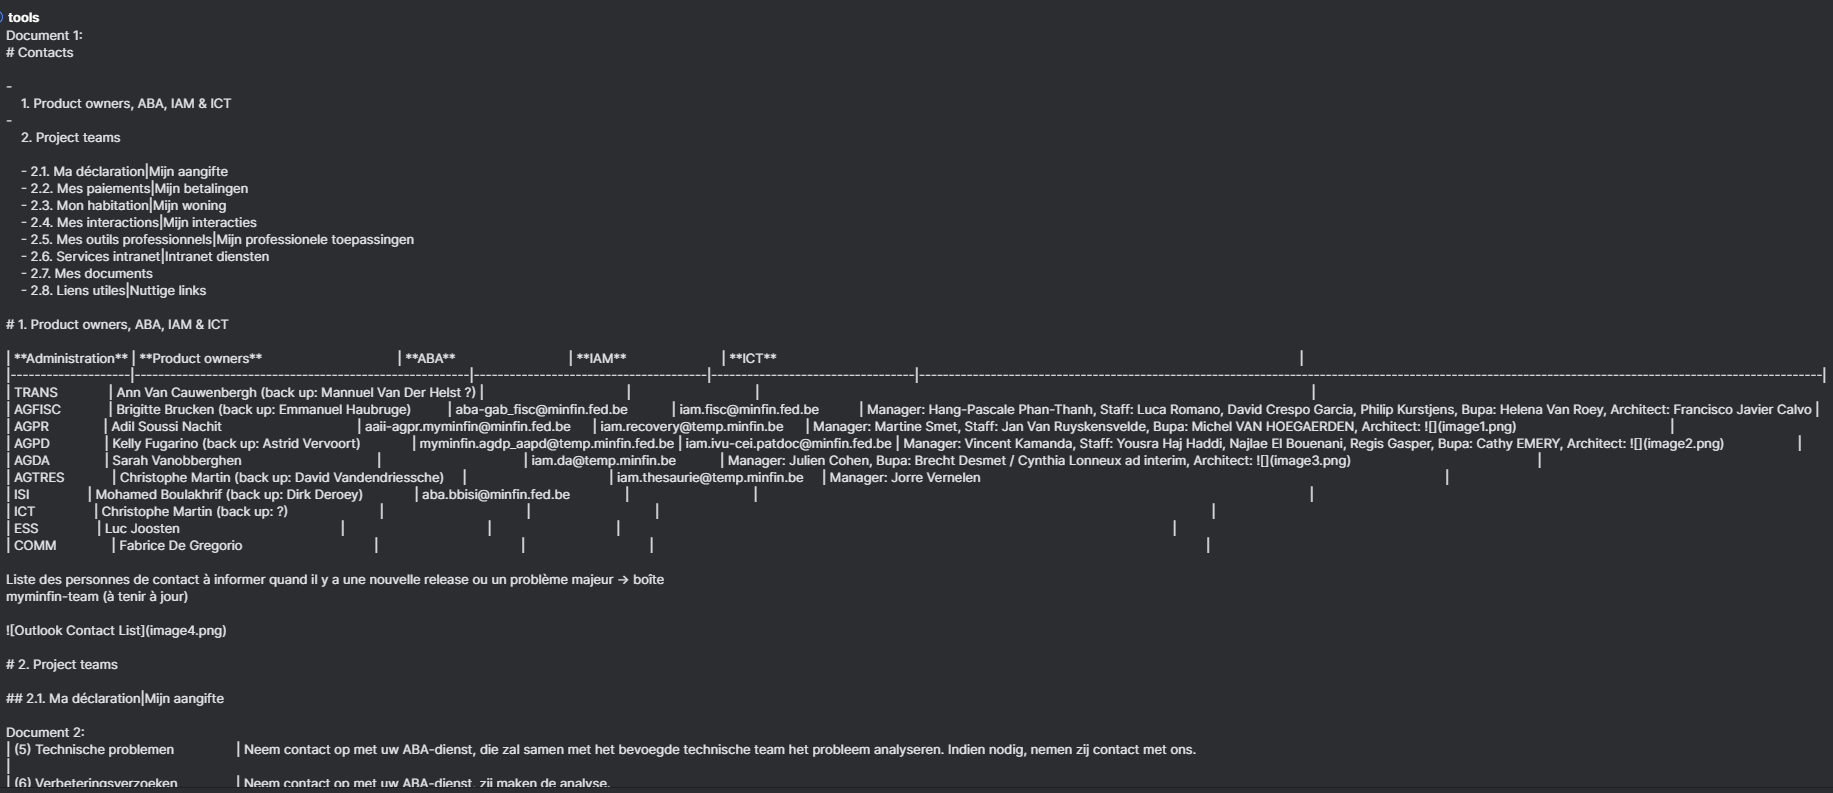
\includegraphics[width=\linewidth]{chunks_md.png}
        \caption{Chunks in Markdown}
        \label{fig:chunks_md}
    \end{subfigure}
    \caption{Drie figuren naast elkaar ter illustratie}
    \label{fig:driefiguren}
\end{figure}


%Hoe heb je dat opgelost? Eventueel kort uitleggen als dat relevant is.

\section{Samenvatting}

%Korte recap: wat is gebouwd en werkt zoals verwacht?

%Eventueel: wat is nog niet geïmplementeerd en waarom niet (scope, tijdsbeperkingen)?

Wat nog niet werd geïmplementeerd maar wel handig zou zijn is om de agent de mogelijkheid te geven om de documentatie te gaan aanpassen. Dit zou ervoor zorgen dat de documentatie steeds up to date zou zijn en er niet langer zelf de aanpassingen zouden moeten doen. Dit is echter een functionaliteit die buiten scope ligt en wegens tijdsgebrek niet meer kon worden aangeleverd binnen deze POC.